% Section 1: Trench Warfare in WWI
%---------------------------------------------------------------------------

\begin{frame}{Trench Warfare in WWI}
  \begin{itemize}
    \item On the Western Front, 
    early advances ground to a halt and stagnated into trench warfare
    \item Technologies like artillery and machine guns made the war one of the bloodiest in human history
  \end{itemize}
\end{frame}

\begin{frame}{Trench Warfare in WWI}
  \begin{center}
    \begin{tabular}{*{4}{c|}}
      \multicolumn{2}{c}{} & \multicolumn{2}{c}{German soldiers} \\ \cline{3-4}
      \multicolumn{1}{c}{} &    & Kill & Miss \\ \cline{2-4}
      \multirow{2}*{Allied Soldiers} & Kill & 2, 2 & 6, 0 \\ \cline{2-4}
                         & Miss & 0, 6 & 4, 4 \\ \cline{2-4} 
    \end{tabular} 
  \end{center}
  What's the \textbf{NE}?
\end{frame}

\begin{frame}{Unexpected Truces Emerge}
  Christmas Day Truce, 1914:
  \begin{center}
    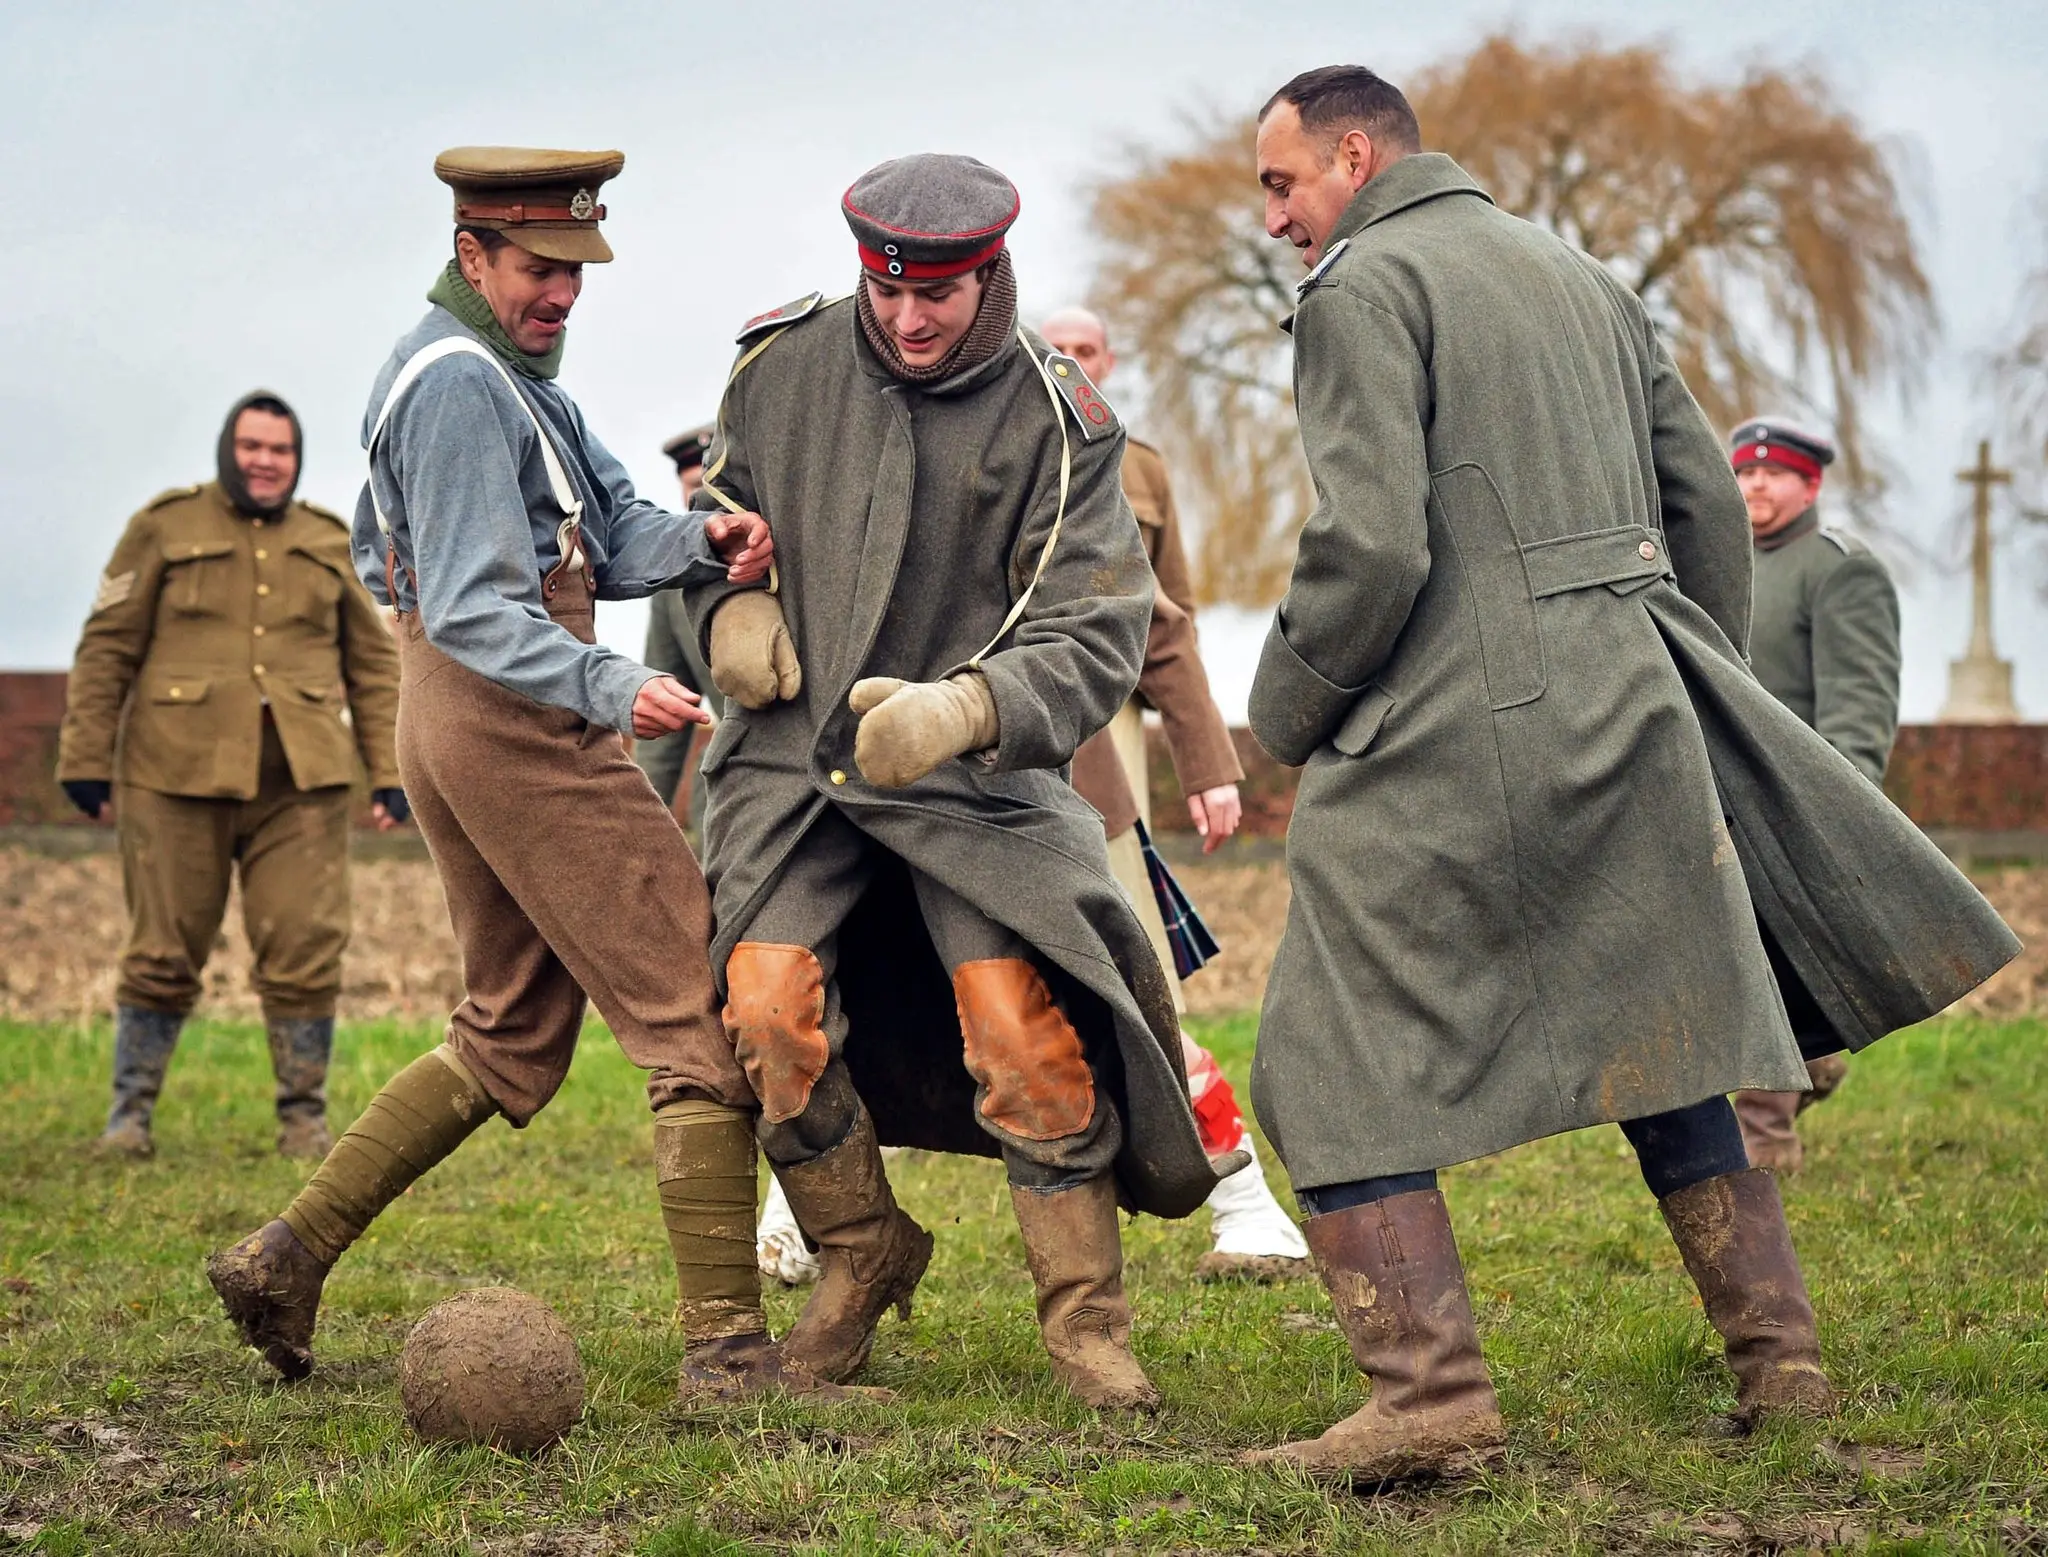
\includegraphics[width=.75\textwidth]{figures/hughes24-superJumbo.png} 
  \end{center}
  {\tiny Image Credit: Stephanie Lecocq/European Pressphoto Agency}
\end{frame}

\begin{frame}{Unexpected Truces Emerge}
  \begin{itemize}
    \item Despite the conditions of war, unexpected truces emerged
    \item Five months after hostilities began, soldiers from opposing sides 
    ventured into no man's land to break bread, bury their dead, and exchange prisoners
    \item other examples of ``\href{https://en.wikipedia.org/wiki/Live_and_let_live_(World_War_I)}{Live and let live}''
    \begin{itemize}
      \item Some soldiers would shoot across the trenches at predictable intervals
      \item refuse to shoot at supply lines
      \item some soldiers refused to fire their weapons at all
    \end{itemize}
  \end{itemize}
\end{frame}

\begin{frame}{The puzzle of trench truces}
  \begin{itemize}
    \item How did cooperation between enemy armies achieved and sustained?
    \item One answer might be that in these parts of the front, interactions were \textbf{repeated} between the same units
  \end{itemize} 
\end{frame}

\begin{frame}{Constructing a Repeated Game}
  Suppose that Allied and German forces anticipate that they will play this game $T$ times 
  \begin{center}
    \begin{tabular}{*{4}{c|}}
      \multicolumn{2}{c}{} & \multicolumn{2}{c}{German soldiers} \\ \cline{3-4}
      \multicolumn{1}{c}{} &    & Kill & Miss \\ \cline{2-4}
      \multirow{2}*{Allied Soldiers} & Kill & 2, 2 & 6, 0 \\ \cline{2-4}
                         & Miss & 0, 6 & 4, 4 \\ \cline{2-4} 
    \end{tabular} 
  \end{center}
  \begin{itemize}
    \item A \textit{strategy} will be made up of $T$ \textit{actions}; 
    one for each time this stage game is played
  \end{itemize}
\end{frame}

% \begin{frame}{Constructing a Repeated Game}
%   To represent this as an extensive form tree, lets suppose that $T=2$:
%   \begin{itemize}
%     \item If neither side sees what their opponent's strategy was yesterday, each player has 3 info sets
%     \item So each side has eight possible strategies:
%     \begin{itemize}
%       \item (\textit{Kill$_1$}, \textit{Kill$_2$} if \textit{Kill$_1$} or \textit{Miss$_1$})
%       \item (\textit{Kill$_1$}, \textit{Kill$_2$} if \textit{Kill$_1$} else \textit{Miss$_2$} if \textit{Miss$_1$})
%       \item (\textit{Kill$_1$}, \textit{Miss$_2$} if \textit{Kill$_1$} else \textit{Kill$_2$} if \textit{Miss$_1$})
%       \item (\textit{Kill$_1$}, \textit{Miss$_2$} if \textit{Kill$_1$} or \textit{Miss$_1$})
%       \item ...
%     \end{itemize}
%   \end{itemize}
% \end{frame}

% \begin{frame}{Constructing a Repeated Game}
%   \begin{center}
%     \includegraphics[width=1\textwidth]{figures/fig132.png} 
%   \end{center} 
% \end{frame}

\begin{frame}{Constructing a Repeated Game}
  To represent this as an extensive form tree, lets suppose that $T=2$:
  and suppose that the history of all past plays are \textbf{common knowledge} 
  \begin{itemize}
    \item each player will have five info sets; one for day 1, and four in day 2 
    \item What does the extensive form game look like?
  \end{itemize}
\end{frame}

\begin{frame}{2-period Prisoners' Dilemma}
  \begin{center}
    \includegraphics[width=1\textwidth]{figures/fig133.png} 
  \end{center} 
  What is the SPNE?
\end{frame}

\begin{frame}{$T$-period Prisoners' Dilemma}
  Suppose that we are already at the last period $T$ of the $T$-period trench warfare game 

  Suppose that the Allies total payoff stream value so far is $A^{T-1}$ and the Germans is $G^{T-1}$ 
  \begin{center}
    \includegraphics[width=.7\textwidth]{figures/tab137.png} 
  \end{center}
  What will happen?
  \pause

  \begin{itemize}
      \item Allies will Shoot to \textbf{Kill},
      Germans will Shoot to \textbf{Kill}
  \end{itemize}
\end{frame}

\begin{frame}{Backwards induction w/ $T$ periods}
  Now that we know the $T$ stage will end in $(Kill_T, ~Kill_T)$, we can look one period back to what will happen in $T-1$: 
  \begin{center}
    \includegraphics[width=.7\textwidth]{figures/fig138.png}
  \end{center}
  What will happen?
  \pause
  \begin{itemize}
      \item Both will shoot to \textbf{Kill} in $T-1$, knowing they will both shoot to kill in $T$
  \end{itemize}
\end{frame}

\begin{frame}{Trench Game with Finite stages}
  By now, you should get the idea:
  \begin{block}{Insight}
    If the stage game has a unique NE, then any finitely repeated version will
    have a unique SPNE which is just the repetition of the single-stage NE. No
    cooperation is sustainable 
  \end{block}

  So what was going on with those spontaneous truces?
\end{frame}

\begin{frame}{Infinitely Repeated Trench Game}
  \begin{itemize}
    \item The problem with that last equilibrium we found was that you have to
      know \textit{exactly when the game will end} to use backwards induction 
    \item But for World War I infantrymen, they didn't know how long it would
      be until the fronts shifted or their division was rotated out
    \item We will have to extend our models to allow for 
      \alert{indefinite horizons}
  \end{itemize} 
\end{frame}


\begin{frame}{Repeated Prisoners' Dilemma with Uncertain Second Stage}
  Suppose that the first stage of the game is the Trenches Game:
  \begin{table}[!h]
    \centering
    \begin{tabular}{*{4}{c|}}
      \multicolumn{2}{c}{} & \multicolumn{2}{c}{German soldiers} \\ \cline{3-4}
      \multicolumn{1}{c}{} &    & Kill & Miss \\ \cline{2-4}
      \multirow{2}*{Allied Soldiers} & Kill & 4, 4 & 8, 2 \\ \cline{2-4}
                         & Miss & 2, 8 & 6, 6 \\ \cline{2-4} 
    \end{tabular} 
  \end{table}
  But with probability $p$, the game repeats in the second round 
  and with probability $1-p$, it ends after the first round
\end{frame}

\begin{frame}{Repeated Prisoners' Dilemma with Uncertain Second Stage}
  Consider the following strategy: 
  \begin{align*}
    \begin{cases}
      \text{In stage } 1 & : \textit{Miss}_1 \\ 
      \text{In stage } 2 & : 
      \begin{cases}
        \textit{Miss}_2 \text{  if the other player Missed in stage 1} \\ 
        \textit{Kill}_2 \text{  if the other player Killed in stage 1}
      \end{cases}
    \end{cases}
  \end{align*}
  Let's call this strategy \textit{Punisher} because it starts off friendly, 
  but will try to punish someone who defects in the first round by defecting in the second round.
\end{frame}

\begin{frame}{Repeated Prisoners' Dilemma with Uncertain Second Stage}
  Suppose you are playing against a \textit{Punisher} in this game. 

  \begin{center}
    \begin{tabular}{*{4}{c|}}
      \multicolumn{2}{c}{} & \multicolumn{2}{c}{German soldiers} \\ \cline{3-4}
      \multicolumn{1}{c}{} &    & Kill & Miss \\ \cline{2-4}
      \multirow{2}*{Allied Soldiers} & Kill & 4, 4 & 8, 2 \\ \cline{2-4}
                         & Miss & 2, 8 & 6, 6 \\ \cline{2-4} 
    \end{tabular} 
  \end{center}

  \begin{itemize}
    \item What is your \textbf{expected utility} of playing $Kill_1, ~Kill_2$?
    \pause
    \item 8 in the first stage, 4 in the second stage,
    \item so $EU(Kill,~Kill) = 8 + 4p$
  \end{itemize}
\end{frame}

\begin{frame}{Repeated Prisoners' Dilemma with Uncertain Second Stage}
  Suppose you are playing against a \textit{Punisher} in this game. 

  \begin{center}
    \begin{tabular}{*{4}{c|}}
      \multicolumn{2}{c}{} & \multicolumn{2}{c}{German soldiers} \\ \cline{3-4}
      \multicolumn{1}{c}{} &    & Kill & Miss \\ \cline{2-4}
      \multirow{2}*{Allied Soldiers} & Kill & 4, 4 & 8, 2 \\ \cline{2-4}
                         & Miss & 2, 8 & 6, 6 \\ \cline{2-4} 
    \end{tabular} 
  \end{center}

  What is your \textbf{expected utility} of playing $Miss_1, ~Kill_2$? \\
  \pause
  \begin{itemize}
      \item $4 + 8p$
  \end{itemize}
  What about from playing \textit{Kill, Miss?} \\
  \pause
  \begin{itemize}
      \item $8 + 2p$
  \end{itemize}
  Would you rather defect earlier or later?
\end{frame}

\begin{frame}{Repeated Prisoners' Dilemma with Uncertain Second Stage}
  Suppose you are playing against a \textit{Punisher} in this game. 

  \begin{center}
    \begin{tabular}{*{4}{c|}}
      \multicolumn{2}{c}{} & \multicolumn{2}{c}{German soldiers} \\ \cline{3-4}
      \multicolumn{1}{c}{} &    & Kill & Miss \\ \cline{2-4}
      \multirow{2}*{Allied Soldiers} & Kill & 4, 4 & 8, 2 \\ \cline{2-4}
                         & Miss & 2, 8 & 6, 6 \\ \cline{2-4} 
    \end{tabular} 
  \end{center}

  What is your \textbf{expected utility} of playing \textit{Miss, Miss}?
  \begin{itemize}
      \item $6 + 6p$
  \end{itemize}
\end{frame}

\begin{frame}{Repeated Prisoners' Dilemma with Uncertain Second Stage}
  Let's graph your expected utilties of each strategy:
  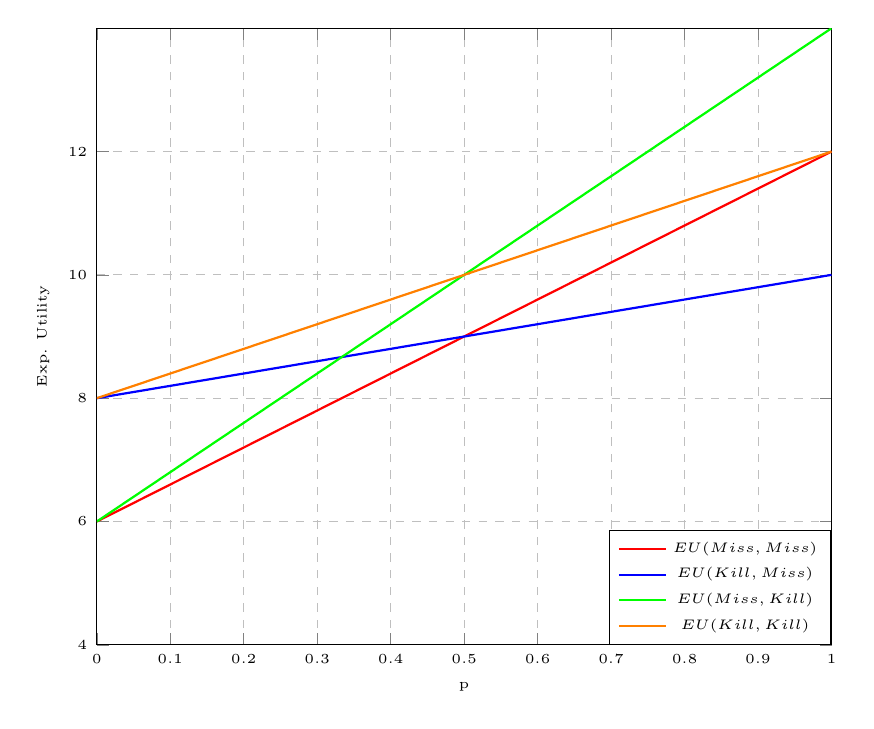
\begin{tikzpicture}
   \begin{axis}[
     width=0.9\textwidth,
     grid,
     xlabel={p},
     ylabel={Exp. Utility},
     xmin=0, xmax=1.0,
     ymin=4, ymax=14,
     xtick={0,.1,...,1.0},
     ytick={2, 4, 6, 8, 10, 12},
     grid style=dashed,
     font=\tiny,
     legend style={at={(1,0)},anchor=south east},
     ]
 
     \addplot[domain=0:1, samples=100, thick, red] {6 + 6*x};
     \addlegendentry{$EU(Miss, Miss)$}

     \addplot[domain=0:1, samples=100, thick, blue] {8 + 2*x};
     \addlegendentry{$EU(Kill, Miss)$}

     \addplot[domain=0:1, samples=100, thick, green] {6 + 8*x};
     \addlegendentry{$EU(Miss, Kill)$}
     
     \addplot[domain=0:1, samples=100, thick, orange] {8 + 4*x};
     \addlegendentry{$EU(Kill, Kill)$}

   \end{axis}
 \end{tikzpicture}
\end{frame}

\begin{frame}{Repeated Prisoners' Dilemma with Uncertain Second Stage}
  With probabalistic 2nd stage:
  \begin{itemize}
    \item players are incentivized to $Miss$ in the first stage if punishment is likely enough
    \item but still not sufficient to incentivize anyone to $Miss$ in the second stage
    \item what if there are \textit{infinite} stages?
  \end{itemize}
\end{frame}

\begin{frame}{Constructing a Repeated Game}
  Let's generalize what a strategy in \textit{any} \alert{repeated game} with \alert{common knowledge} will look like:
  \begin{itemize}
    \item If a game has $T$ periods, and each player has $m$ actions at each stage,
    \item there is one initial info set, $m^2$ info sets in period 2, $m^4$ info sets in period 3, ..., $m^{2(T-1)}$ in the last period 
    \item A complete strategy is made up of $1 + m^2 + m^4 + ... + m^{2(T-1)}$ actions 
  \end{itemize}
  In an \alert{infinitely repeated game}, there will be an infinite number of actions in each strategy
\end{frame}

\begin{frame}{Constructing a Repeated Game}
  How to model streams payoffs over time?
  \begin{itemize}
    \item We could just add up all of the per-stage payoffs across an entire history
    \item But for infinitely-long histories, this sum would blow up and not make much sense
    \item Instead, we will use \alert{present value} calculations
  \end{itemize}
\end{frame}

\begin{frame}{Present Values}
  Suppose that I have an income stream where I earn $w_t$ dollars in every year $t$
  \begin{itemize}
    \item The \alert{interest rate} $r$ is how much I could earn each year on a risk-free bond
    \item My present value over my whole income stream is 
    $$ w_1 + \frac{w_2}{(1+r)} + \frac{w_3}{(1+r)^2} + \frac{w_4}{(1+r)^3} + ... + \frac{w_T}{(1+r)^{T-1}} $$
    \item This represents the value I place on this income stream vs having the interest from the payment up front
    \item Money today is worth more than money tomorrow
  \end{itemize}
\end{frame}

\begin{frame}{Infinitely Repeated Games}
  Suppose the probability that at each stage, with probability $p$, the game continues and with $(1-p)$, the game ends and you get $u=0$

  The \textbf{expected present value} of a stream of payoffs $u_1, u_2, ...$ is then:
  $$ V = u_1 + \frac{p u_2}{(1+r)} + \frac{p^2 u_3}{(1+r)^2} + ... = \sum_{t=1}^{\infty}\left(\frac{p}{(1+r)}\right)^{t-1}u_t $$
\end{frame}

\begin{frame}{Infinitely Repeated Games}
  Now if we let $\delta = \frac{p}{(1+r)}$ represent the \alert{subjective discount factor}
  $$ V = \sum_{t=1}^{\infty}(pd)^{t-1}u_t = \sum_{t=1}^{\infty}\delta^{t-1}u_t $$
  \begin{itemize}
    \item $\delta$ captures discounting from uncertainty and present value
  \end{itemize}
\end{frame}

\begin{frame}{Present Values}
  What about calculating a present value of an \alert{infinte stream} of payoffs?
  \begin{itemize}
    \item It turns out:  
    $$ x + \delta x + \delta^2 x + \delta^3 x + ... + \delta^{\infty} x $$
    \item actually converges to $\frac{x}{1-\delta}$ as long as $\delta<1$ 
  \end{itemize}
\end{frame}

\begin{frame}{SPNE in Repeated Games}
  A strategy profile is SPNE if and only if in each period and for each history, the prescribed action is optimal given:
  \begin{itemize}
    \item the other players act according to their strategies in the current period
    \item all players act according to their strategies in all future periods
  \end{itemize}
\end{frame}

\begin{frame}{Grim Trigger in the Trench Game}
  Consider the following strategy: 
  \begin{itemize}
    \item In period 1, choose miss
    \item In period $t>1$, choose miss if both chose miss in all past periods, else choose kill
  \end{itemize}
  This type of strategy is known as \alert{Grim Trigger} because this type of player starts out cooperative, but if wronged once, they will always shoot to kill
\end{frame}

\begin{frame}{Cooperative Equilibrium in the Trenches}
  Revisiting the Christmas Truce:
  \begin{center}
    \begin{tabular}{*{4}{c|}}
      \multicolumn{2}{c}{} & \multicolumn{2}{c}{German soldiers} \\ \cline{3-4}
      \multicolumn{1}{c}{} &    & Kill & Miss \\ \cline{2-4}
      \multirow{2}*{Allied Soldiers} & Kill & 4, 4 & 8, 2 \\ \cline{2-4}
                         & Miss & 2, 8 & 6, 6 \\ \cline{2-4} 
    \end{tabular} 
  \end{center}
  \begin{itemize}
    \item Suppose that the Allies play the Grim Trigger Strategy
    \item When will the Germans want to Miss?
    \pause
    \begin{itemize}
      \item when $pv(\text{Kill always}) < pv(\text{Miss always})$
      \item $pv(Kill always) = 8 + 4\delta + 4 \delta^2 + ... $
      \item $pv(Miss always) = 6 + 6\delta + 6 \delta^2 + ... $
      \item So Cheat when $ 8 + \frac{4\delta}{1-\delta} < 6 + \frac{6\delta}{1-\delta}$
      \item or when $\delta > \frac{1}{2}$
    \end{itemize}
  \end{itemize}
\end{frame}

\begin{frame}
  \frametitle{Tit for Tat in the Trench Game}
  \begin{itemize}
    \item In period 1, choose miss
    \item In period $t>1$, choose whatever other player chose in $t-1$
  \end{itemize}
  This type of strategy is known as \alert{Tit-for-Tat} because it copies the opponent's previous strategy
\end{frame}

\begin{frame}{SPNE with Tit-for-Tat}
  Revisiting the Christmas Truce:
  \begin{center}
    \begin{tabular}{*{4}{c|}}
      \multicolumn{2}{c}{} & \multicolumn{2}{c}{German soldiers} \\ \cline{3-4}
      \multicolumn{1}{c}{} &    & Kill & Miss \\ \cline{2-4}
      \multirow{2}*{Allied Soldiers} & Kill & 4, 4 & 8, 2 \\ \cline{2-4}
                         & Miss & 2, 8 & 6, 6 \\ \cline{2-4} 
    \end{tabular} 
  \end{center}
  \begin{itemize}
    \item Suppose that the Allies play the Tit-for-Tat
    \item When will the Germans want to Kill once? (and then go back to Missing?)
    \pause
    \begin{itemize}
      \item when $pv(Cheat) < pv(Coop)$
      \item $pv(Cheat) = 8 + 2\delta + 6 \delta^6 + ... $
      \item $pv(Coop) = 6 + 6\delta + 6 \delta^2 + ... $
      \item So Kill once when $ 8 + 2\delta + 6\sum_{t=3}^\infty \delta^{t-1} < 6 + 6\delta + 6\sum_{t=3}^\infty \delta^{t-1}$
      \item or when $\delta > \frac{1}{2}$
    \end{itemize}
  \end{itemize}
\end{frame}

\begin{frame}{Cooperative Equilibrium in the Trenches}
  Revisiting the Christmas Truce:
  \begin{itemize}
    \item SPNE is achieved using both strategy (Grim Trigger or Tit-for-Tat)
    \item as long as player have discount rate $\delta > \frac{1}{2}$
    \item interpret this as more patient $\rightarrow$ more likely to cooperate
    \item alternatively, the more likely is future repeated play
    \begin{itemize}
      \item what happened in the trenches as both sides started to cycle troops more often?
      \item when will cooperative repeated games equilibria break down?
    \end{itemize}
  \end{itemize}
\end{frame}
